\documentclass[12pt,a4paper]{article}
\usepackage[utf8]{inputenc}
\usepackage[francais]{babel}
\usepackage[T1]{fontenc}
\usepackage{amsmath}
\usepackage{amsfonts}
\usepackage{amssymb}
\usepackage{float}
\usepackage[left=2cm,right=2cm,top=2cm,bottom=2cm]{geometry}
\usepackage{graphicx}
\usepackage{tabularx}

\bibliographystyle{alpha}

\newcommand{\HRule}{\rule{\linewidth}{0.5mm}}

\begin{document}
%%% Page de garde %%%
\begin{titlepage}
\begin{center}


\includegraphics[width=0.3\textwidth]{images/universite_bordeaux_logo.pdf}\\[1cm]    

\textsc{\LARGE Université de Bordeaux}\\[1.5cm]

\textsc{\Large Projet de Programmation}\\[0.5cm]

\vspace{30pt}
% Title
\HRule \\[0.4cm]
{ \huge \bfseries VisualMapReduce}\\[0.4cm]

\HRule \\[1.5cm]

% Author and supervisor
\begin{minipage}{0.4\textwidth}
\begin{flushleft} \large
\textbf{Auteurs :}\\
Kinda \textsc{Al Chahid}\\
Marc-Alexandre \textsc{Espiaut}\\
Imen \textsc{Hentati}\\
Oualid \textsc{Yjjou}
\end{flushleft}
\end{minipage}
\begin{minipage}{0.4\textwidth}
\begin{flushright} \large
\textbf{Client :} \\
Alexandre \textsc{Perrot}\\
\textbf{Chargé de TD :} \\
Maria \textsc{Predari}
\end{flushright}
\end{minipage}

\vfill

% Bottom of the page
{\large \today}

\end{center}

\end{titlepage}

%%% FIN Page de garge %%%

\tableofcontents
\newpage
\section{Introduction}
Avec l'augmentation du volume de données à traiter, le BigData est une problématique qui s'est progressivement introduite en entreprise.\cite{JoliaFerrierBigData} MapReduce est un algorithme qui tente d'apporter une réponse satisfaisante au traitement d'un grand volume de donnée. Il est notamment utilisé par Google pour son algorithme de recherche, mais aussi par d'autres entreprises (telles que Facebook, IBM, ..).
\paragraph{}
L'exécution d'un programme MapReduce se fait sur un cluster\footnote{Un \textit{cluster} est une grappe de machines sur un réseau.} contenant généralement un grand nombre de machines, ce qui rend le débogage compliqué. En effet, si une des machines ne parvient pas à exécuter le programme correctement, le retour n'est pas fait à l'utilisateur et l'identification de l'origine du problème est difficile.
Le but de VisualMapReduce est de simuler le fonctionnement d'un programme MapReduce sur un cluster de machines afin de pouvoir le tester avant son application dans le monde réel pour éviter ce genre de problèmes.

Cette application, destiné à l'enseignement, permettra à des étudiants en Master 2 Informatique de simuler et comprendre le fonctionnement de MapReduce.
\paragraph{}
Dans le cadre de notre projet de programmation, nous devons travailler sur la visualisation d'un cluster exécutant du code de MapReduce via une application web, c'est à dire une représentation graphique du cluster accompagné d'un affichage individuel par machine du code MapReduce en cours d'exécution pour repérer facilement la provenance d'un bogue.
MapReduce est un pradigme de programmation servant à traiter et à générer de grands jeux de données avec un algorithme distribué et parallelisé sur un cluster.\\
 MapReduce \cite{Bdpedia} décrit deux tâches séparées ; la tâche \texttt{map()} qui converti un jeu de donnée A en un jeu de donnée B, où les éléments individuels sont découpés en tuples (paire clé/valeur), et la tâche reduce() prends en entrée le résultat produit par map() pour combiner les tuples de données produites en un plus petit jeu de tuples.
Comme le nom MapReduce l'indique, la tâche \texttt{reduce()} s'effectue toujours après la tâche \texttt{map()}.
\paragraph{}
%L'algorithme MapReduce est utilisé pour gérer des bases de données avec d'importante quantité de donnée. Ainsi, plusieurs entreprises utilise le MapReduce de Google tel que FaceBook\cite{ApacheWikiFacebook} qui l'utilise pour analyser ses données dans le but d'améliorer et signaler des données mais également pour du machine learning.
\newpage


\subsection{Description du process de MapReduce}
L'algorithme MapReduce se décompose en plusieurs phases: {\tt Map, Combine, Partitioner, Shuffle} et {\tt Reduce}.\\
\begin{itemize}
\item {\tt Map}: Prend en entrée une ou plusieurs données. Les résultats sont stockés sous forme de <key, value> (<clé, valeur>) dits intermédiaires.

\item {\tt Combine}: Optionnel. Il possède les mêmes propriétés d'entrée/sortie que map. Son but est de faciliter la tâche de reduce en efectuant un "merge" partiel\cite{Google} sur les résultats du map.

\item {\tt Partitioner}: contrôle le partitionnement des clés des résultats de map. Par défaut, le partitioner utilise une fonction de hashage.Le nombre total de partitions est le même que le nombre des tâches de reduce. 


\item {\tt Shuffle}: C'est la phase de transfert des données des mappers aux reducers. Plus clairement, elle fournie les entrées de reduce.

\item {\tt Reduce}: C'est la phase de calcul du process. Elle accepte les clés intermédiaires et un ensemble de valeurs d'une même clé. Les valeurs sont alors traitées selon la fonction {\tt reduce} fournie.
\end{itemize}

\begin{figure}[H]
  \centering
    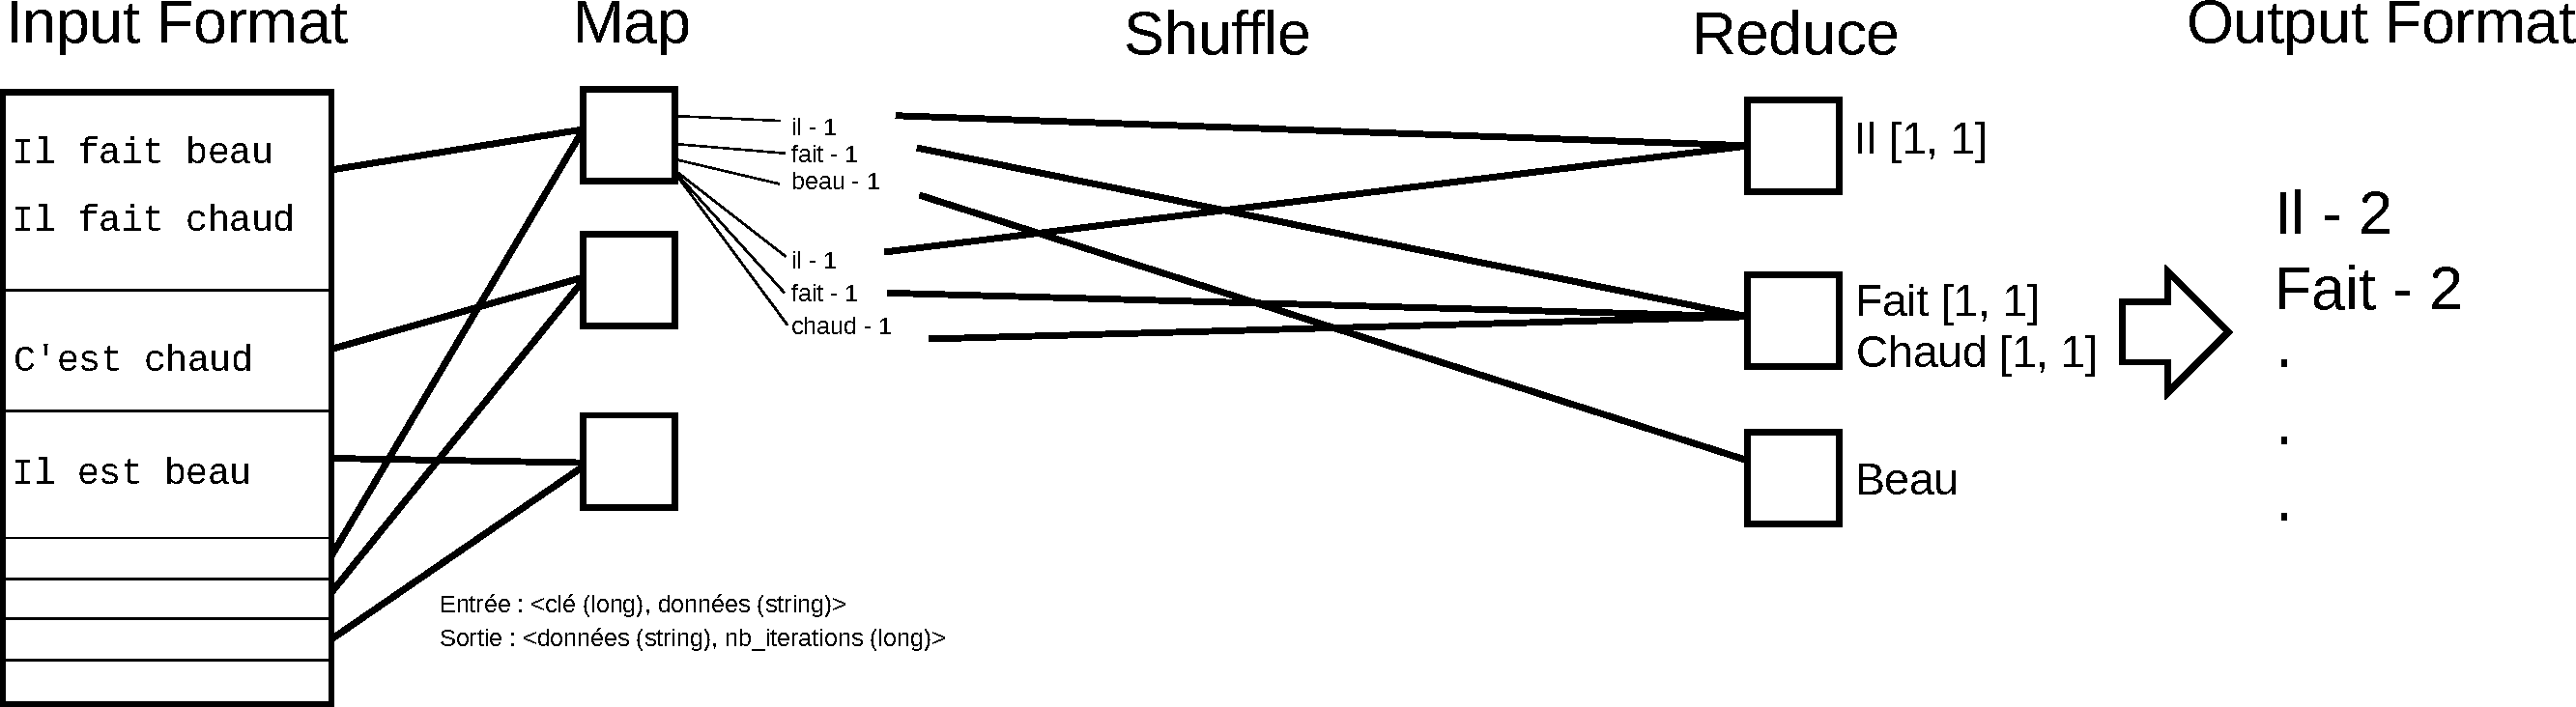
\includegraphics[scale=0.3]{images/shuffle_explication.pdf}
        \caption{Schéma MapReduce}
\end{figure}

\section{But de ce document}

Après discussion avec le client, nous avons pris connaissance des ses
besoins, ses priorités et ses attentes. 

Ce document nous permet d'avoir
une première réflexion sur le projet, le fonctionnement global du
logiciel, la priorité des étapes, et leurs faisabilité dans le temps
imparti. 

Ce cahier des besoins nous permet de rédiger et d'organiser les
demandes de notre client, et pourra être repris par une autre équipe afin
d'en continuer le développement.
\section{But du projet}\label{but-du-projet}

Le but de notre projet est de réaliser un interpréteur MapReduce \cite{Google} afin de
pouvoir en visualiser, par une application web, le fonctionnement de cet algorithme en montrant les différentes connexions entre map et reduce dans un cadre pédagogique.

L'exécution se fera localement dans le navigateur, et n'aura pas besoin de communiquer avec une base de données.
\section{Public visé}

\textbf{Pour qui ?} Pour l'enseignant et ses étudiants de Master 2 Informatique de l'Université de Bordeaux.

\textbf{Dans quel but ?} Offrir une plateforme pour visualiser et configurer l'exécution d'un code MapReduce sur un ensemble de données. 

\textbf{Entrée/Sortie} - Fichier \texttt{.csv} (jeu de données) - Paramètre du cluster - Code (Fonctions \texttt{map()} et \texttt{reduce()} pour traiter les données). En sortie: Simulation du process sous forme graphique - Fichier \texttt{.csv} des résultats (à télécharger).

\newpage
\section{Analyse des besoins}
\subsection{Besoins fonctionnels}
\subsection{Besoins essentiels}

%Hierarchisation: selon les phases du projet %%%%%%%%%%%%

\subsubsection{Importation}

\textbf{• Importer un fichier de données (sous format csv)\\} L'utilisateur choisit parmi sa propre bibliothèque de fichiers un fichier sous format {\tt csv} qui contient des lignes de données sur lesquelles il veut appliquer son code mapReduce. L'extension doit être en .csv mais en revanche nous ne limitons pas la taille du fichier (surtout qu'on est dans un contexte de Big Data). Plus de détails sur le fichier est retrouvé dans le chapitre 4 Implémentation.\\

\textbf{• Importer un fichier contenant les fonctions de mapReduce\\}   
 Donner la main à l'utilisateur pour charger son propre code mapReduce avec les 3 fonctions à implémenter "map", "reduce" et "getPartition". Ce sont ces fonctions qui serviront pour le traitement des données en {\tt csv} qu'il a fournit. Le fichier doit donc être sous format {\tt js} mais par contre il n'est pas nécessaire d'en fournir un.\\

\subsubsection{Configuration} 

\textbf{• Configurer le cluster de map\\ } Offrir la possibilité à l'utilisateur de fournir le nombre de machines ainsi que le nombre de coeurs par machine. Par contre, il est limité par un maximum de 20 machines à 24 coeurs chacune pour des raisons expliquées plus tard dans ce document. \\

\textbf{• Configurer le nombre de Reducer du programme\\}  Il est possible de préciser que le code mapReduce sera traité avec un nombre de tâches de reduce (Reduce Task) bien défini. En effet, la simulation peut varier si on a une seule tâche de reduce, dans ce cas toutes les données seront transférées vers un seul {\tt Slot} et le temps de traitement sera plus long. Par contre, utiliser plusieurs reducers permet une bonne parallélisation selon les cas. Pour ce nombre, il est obligatoire de ne pas dépasser le nombre de slots existants dans la phase de map.  \\

\subsubsection{Modification} 

\textbf{• Modifier les fonctions de mapReduce\\} C'est un besoin étroitement lié à "Importer un fichier contenant les fonctions de mapReduce". Quand l'utilisateur joint son fichier .js, celui-ci est directement chargé dans une zone de texte totalement modifiable. Ainsi, il peut voir son propre code contenu dans le fichier mais aussi effectuer directement des modifications dessus sans avoir à l'ouvrir ailleurs dans un éditeur de texte. C'est une fonctionnalité très utile pour pouvoir tester son code sur plusieurs cas et voir à chaque fois la simulation obtenue.  \\

\subsubsection{Visualisation}

\textbf{•  Visualiser la simulation de l'exécution de mapReduce\\} C'est le service principal offert par notre application. Suivant les entrées de l'utilisateur (données csv, code mapReduce en js et configuration du cluster), un graphique est généré en dessous de la zone de code. Il est affiché alors le process de mapReduce selon ses spécifications.\\

\textbf{• Consulter les résultats sur console\\} En plus du graphique, l'utilisateur peut notamment voir les résultats des variables de sorties des différentes phases. Ce besoin est intéressant quand il veut consulter les résultats des phases de partitioner et de shuffle qui ne sont pas inclus dans la simulation graphique pour ne pas allourdir la lisibilité de ce dernier.\\

\textbf{• Consulter les données exécutées sur un slot\\} Une fois la simulation affichée et le graphique généré, on obtient l'ensemble des machines avec leurs différents coeurs ainsi que les liaisons qui montrent la distribution des données. Pour consulter les données exécutées sur un slot en particulier, l'utilisateur clique sur ce slot. Une zone à droite de la page est alors remplie avec les différentes lignes exécutées sur ce map ou bien reduce (un slot peut contenir soit un map soit un reduce).\\ 
 
\subsubsection{Exportation}

\textbf{• Exporter le résultat de la simulation\\} L'utilisateur peut récupérer les données de sortie du process de mapReduce sous forme d'un fichier de données {\tt csv}. Ce fichier contient toutes les lignes de résultats ayant chacune la structure suivante: "clé; valeur".


\subsection{Besoin optionnel}

\textbf{• Exporter les fonctions générées en langage Java\\} Ceci permet d'avoir le code Java du process MapReduce équivalent à celui en Javascript utilisé pour traiter les données. Ce besoin est facultatif en vue du manque de temps que nous puissions rencontrer.

\subsection{Priorité des besoins fonctionnels}
En plus du découpage besoins essentiels/besoins optionnels, nous pouvons indiquer la priorité des besoins. (Voir tableau ci-dessous)
\begin{center}
\begin{tabularx}{\textwidth}{|X|X|}
  \hline {\bf Besoins} & {\bf Priorité attribuée} \\[4ex]

  \hline Importer un fichier des fonctions & Priorité élevée\\[2ex]
  \hline Configurer les fonctions & Priorité élevée\\[2ex]
  \hline Visualiser la simulation & Priorité élevée\\[2ex]
  \hline Importer un fichier de données & Priorité élevée\\[2ex]
  \hline Configurer le cluster de map & Priorité moyenne\\[2ex]
  \hline Consolter données d'un slot & Priorité moyenne\\[2ex]
  \hline Consulter résultats sur console & Priorité faible\\[2ex]
  \hline Configurer le cluster de reduce & Priorité faible\\[2ex]
  \hline Exporter le résultat de la simulation & Priorité faible\\[2ex]
  \hline Exporter les fonctions en java & Priorité faible\\[2ex]
  \hline
\end{tabularx}
\end{center}
\section{Besoins non fonctionnels}



\textbf{Lisibilité du résultat\\} L'utilisateur doit pouvoir lire sans difficulté le résultat du \textit{MapReduce}. Il faut pouvoir zoomer et naviguer dans le graphique réalisé par \textit{FATuM} pour comprendre les liens entre le \textit{mapper} et le \textit{reducer}. L'utilisateur doit pouvoir cliquer sur les slot pour obtenir une liste des données contenues, et ainsi comprendre leurs répartitions.\\

Pour des raisons de visibilité à l'écran et pour simplifier la lecture du graphique, c'est la distribution des données entre map et reduce (avec pour chacun ses entrées et ses sorties) qui est générée. La distribution suit les configurations apportées.

\textbf{Affichage des données dans la console\\} Le résultat des fonctions \texttt{map()} et \texttt{reduce()} doit être affiché dans la console Javascript pour permettre à l'utlisateur d'obtenir le résultat sans avoir à passer par l'interface graphique générée par \textit{FATuM}.


\section{Illustration des besoins}
\subsection{Diagramme de flux de données (DFD)}

\begin{figure}[H]
  \centering
    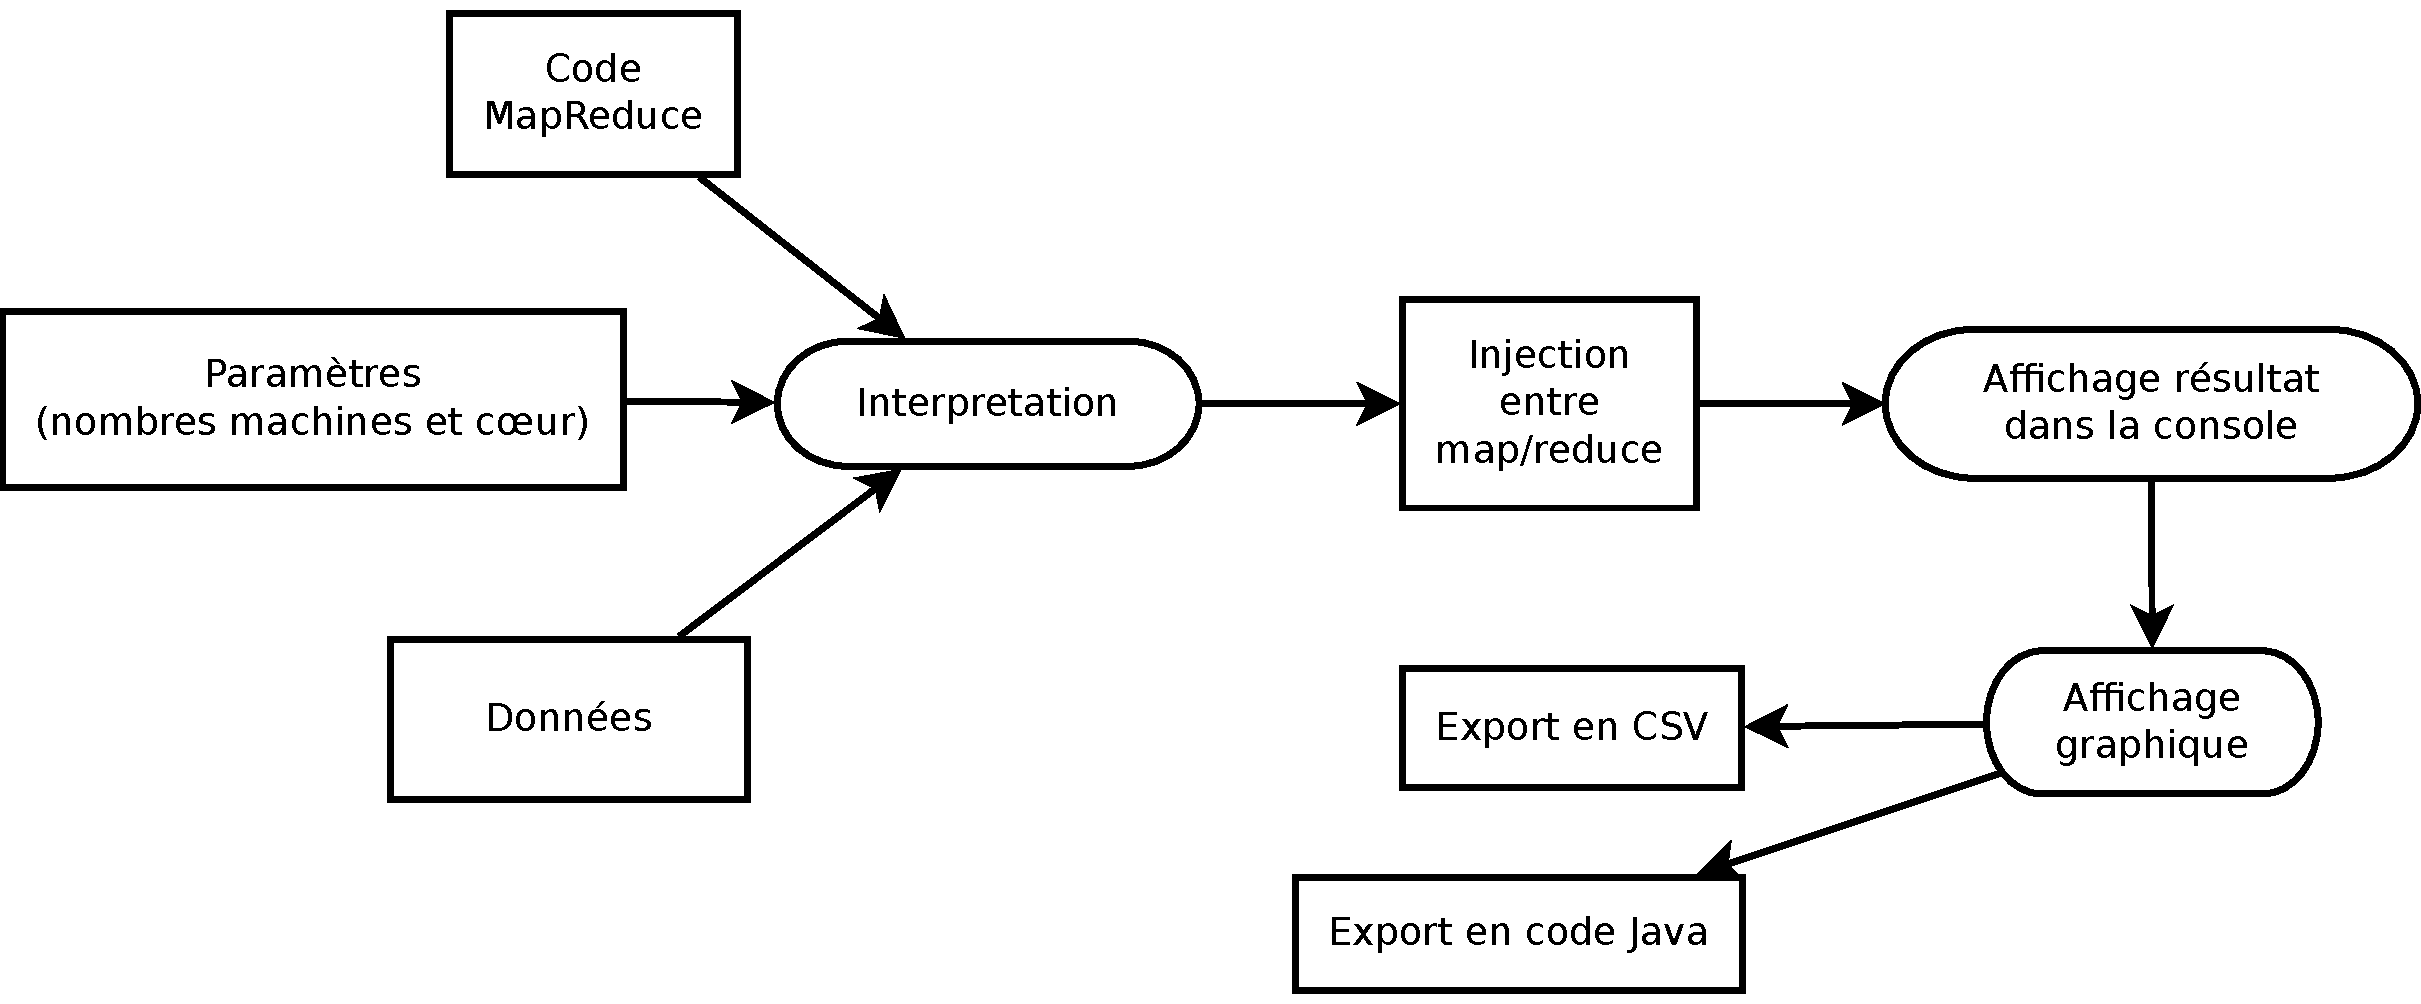
\includegraphics[width=1\textwidth]{images/diagramme_de_flux_de_donnees.pdf}
	\caption{Diagramme de flux de données}
\end{figure}

Le déroulement du programme commence par l'interprétation du code MapReduce en fonction des inputs reçus. Il y a aussi la phase d'injection entre Map et Reduce qui consiste à configurer le cluster et l'adapter selon les critères de l'utilisateur. Pour vérifier le bon fonctionnement de l'interprétation, le résultat est affiché dans la console, ensuite il est généré graphiquement. Il y a possibilité d'exporter les données en CSV ou en langage Java.
\subsection{Diagramme de cas d'utilisation}

\begin{figure}[H]
  \centering
    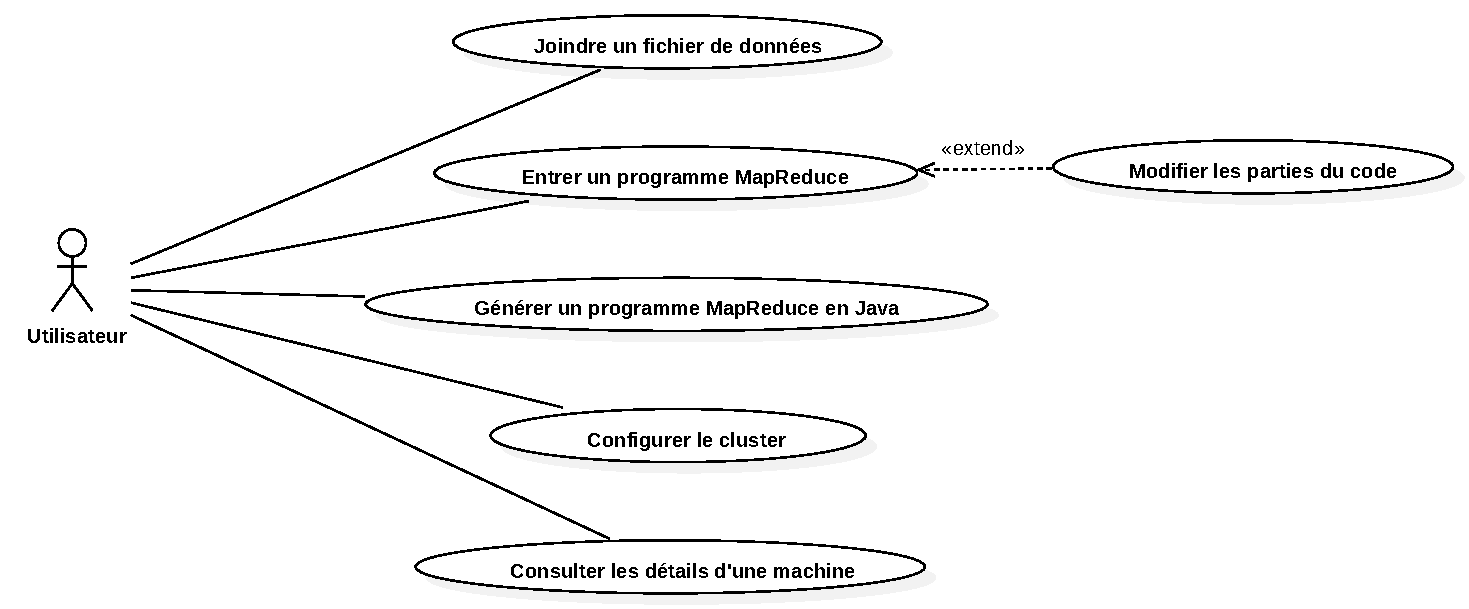
\includegraphics[width=1\textwidth]{images/UseCaseDiagram.pdf}
	\caption{Diagramme de cas d'utilisation}
\end{figure}

Le diagramme de cas d'utilisation permet d'avoir une vision plus claire sur les fonctionnalités de notre programme. En effet, nous avons un seul acteur qui est l'utilisateur et dont les actions possibles sont décrites par les cas d'utilisation illustrés dans la figure ci-dessus.
\subsection{Diagramme de séquence}

\begin{figure}[H]
  \centering
    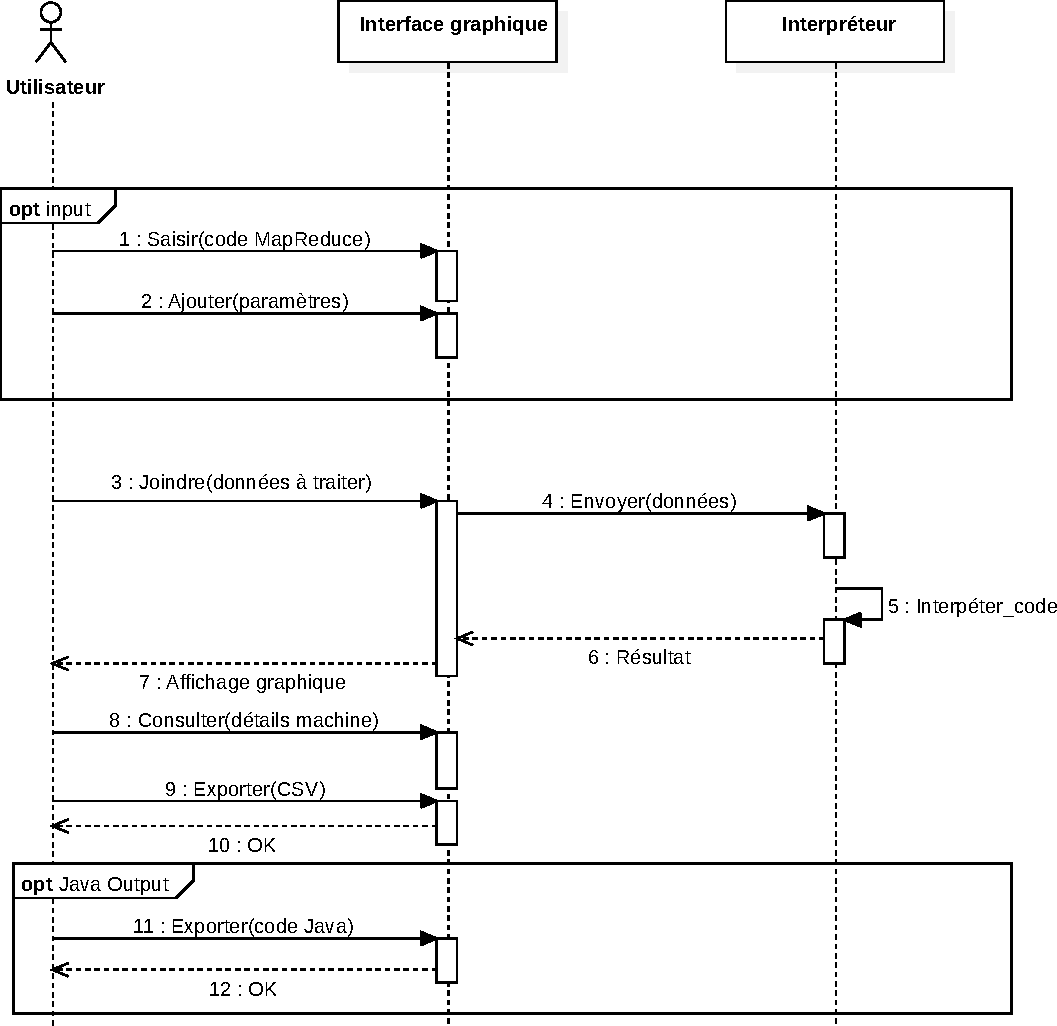
\includegraphics[width=1\textwidth]{images/SequenceDiagram.pdf}
	\caption{Diagramme de séquence}
\end{figure}

Le diagramme de séquence montre les étapes de déroulement du programme. L'utilisateur interagit directement avec l'interface. Le code MapReduce ainsi que les paramètres sont facultatifs. En revanche, il introduit nécessairement les jeux de données.
Les entrées qu'il fournit sont transmises à l'interpréteur qui lui effectue le traitement nécessaire et renvoie un résultat de la simulation. Sur le graphique obtenu, l'utilisateur peut voir la section de données prise en charge par la machine qu'il consulte. La partie d'exportation des données en code Java est optionnelle.


\subsection{Prototypes d'interface}\label{prototypes-interface}
\begin{figure}[H]
  \centering
    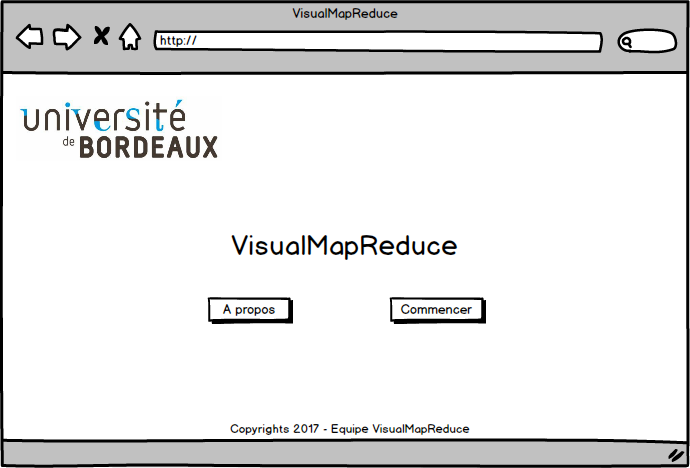
\includegraphics[width=0.75\textwidth]{images/interface/page_accueil.png}
    \caption{Page d'accueil}
\end{figure}

\begin{figure}[H]
  \centering
    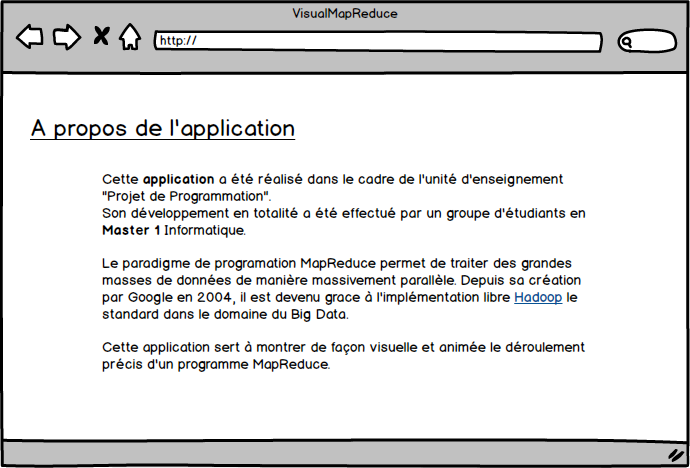
\includegraphics[width=0.75\textwidth]{images/interface/page_a_propos.png}
    \caption{A propos}
\end{figure}

\begin{figure}[H]
  \centering
    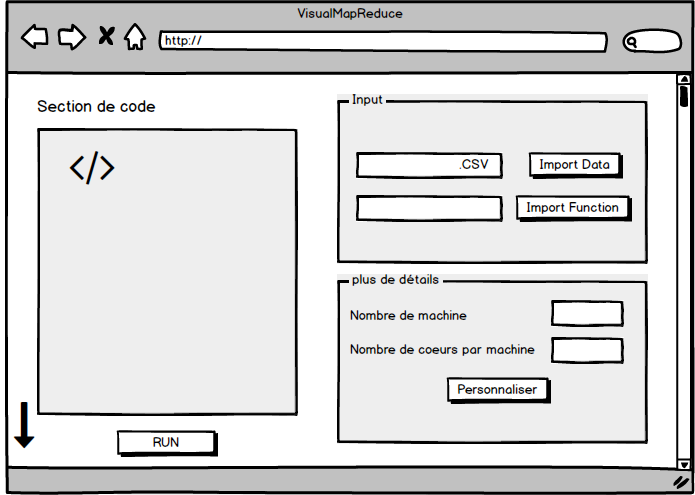
\includegraphics[width=0.75\textwidth]{images/interface/page_interpret1.png}
    \caption{Page d'interprétation}
\end{figure}

\begin{figure}[H]
  \centering
    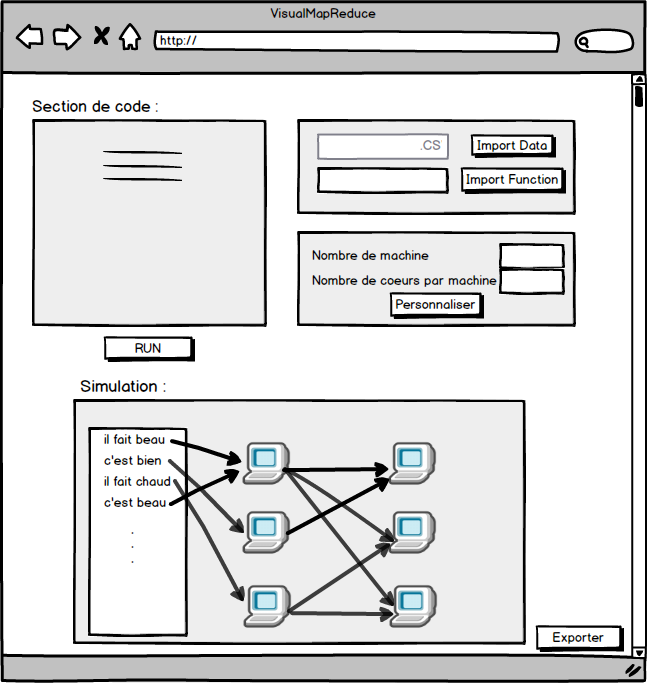
\includegraphics[width=0.75\textwidth]{images/interface/page_interpret2.png}
    \caption{Affichage du résultat}
\end{figure}

L'application étant monopage, le résultat de la simulation est directement affichée sur la même page où l'utilisateur remplit les données. Le graphique apparaît en dessous de la première section.

\begin{figure}[H]
  \centering
    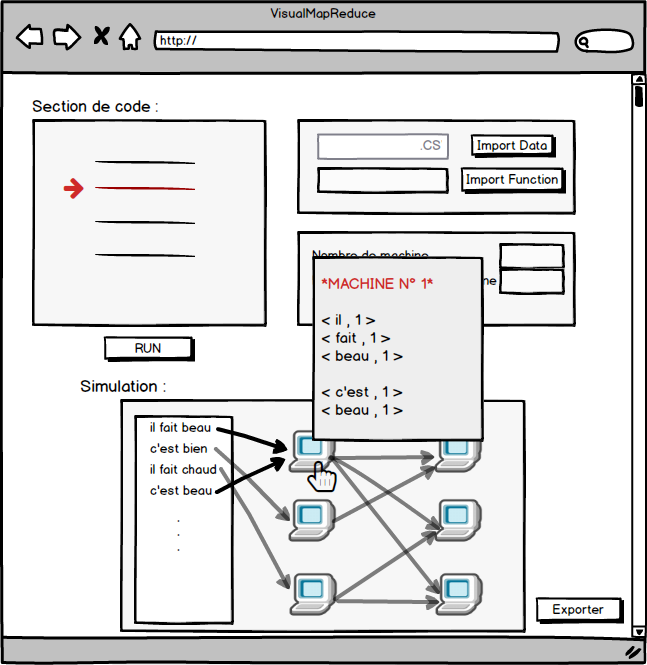
\includegraphics[width=1\textwidth]{images/interface/page_interpret3.png}
    \caption{Détail d'une machine}
\end{figure}

Comme illustré dans la figure ci-dessus, l'utilisateur a la possibilité de consulter les détails d'exécution qui concernent une machine particulière. Ceci permet notamment de résoudre le problème de détection de bogue au sein d'un cluster. Lorsque l'utilisateur appuie sur l'icône de l'une des machines, l'ensemble des propriétés qui concernent celle-ci s'affichent à l'écran. Il peut aussi voir quelle partie de la section de code est exécutée sur cette machine.
\newpage
\section{Tests}
Afin de garantir le bon déroulement du développement du programme et d'identifier rapidement les régressions, nous concevons plusieurs tests de validation.
En voici une liste exhaustive.
\vspace{0.8pt}

\scalebox{0.75}{
\begin{tabular}{|c|c|c|c|}
  \hline
  Entrée & Attendu & Erreurs éventuelles & Importance\\
  \hline
  Code MapReduce & Syntaxe correcte. & Erreurs de syntaxe & Critique.\\
  & Respecte le format imposé. & & Empêche le programme  de se lancer.\\
  \hline
  Données & Fichier .csv & Fichier manquant. & Critique. \\
  & & Données aléatoires. & Empêche le programme de se lancer.\\
  \hline
  Paramètres & Nombre supérieur à zéro. & Nombre inférieur à zéro. & Critique. \\
  & & N'est pas un nombre. & Empêche le programme de se lancer.\\
  & & Manquant. &\\
  \hline
\end{tabular}}

\vspace{10pt}
\begin{itemize}
\item \textbf{Code MapReduce} (\emph{optionnel}) : Code en JavaScript qui comprend les fonctions du Mappeur/Reduceur. Erreurs de syntaxes dûes à l'utilisateur dans son code. Nous ne savons au moment de l'écriture comment prévenir ce problème.

\item \textbf{Données} : Jeux de données sous format \texttt{.csv}.

\item \textbf{Paramètres} (\emph{optionnel}) : Nombre de machines et nombres de cœurs par machine.
\end{itemize}

%% -------------------------------------------------------
\paragraph{Test du résultat de l'interpréteur} ~\\
Afin de vérifier l'adéquation du produit aux exigences fonctionnelles du client, on teste que le produit réalisé est le bon d'une manière textuelle explicative.
Dans ce qui suit le test de la fonction de visualisation de la simulation.
\vspace{11pt}

\begin{tabularx}{\textwidth}{|X|X|X|X|}
  \hline
  Désignation & Condition requise & Démarche à suivre & Résultat attendu\\
  \hline 
  Visualiser la simulation. & Les données initialement sous format CSV sont transformées et affichées dans une section à gauche. Chaque ligne est traitée par une machine. La simulation est affichée et est valide.& Sélectionner une machine du cluster à visualiser en cliquant sur son icône correspondante. & Les données traitées sur la machine sélectionnée apparaissent à l'écran.\\
  \hline
\end{tabularx}
\newpage
\section{Diagramme de Gantt}
Nous illustrons dans cette section la mise en œuvre des besoins décrits précédemment à travers un diagramme de Gantt. 
\begin{figure}[H]
  \centering
    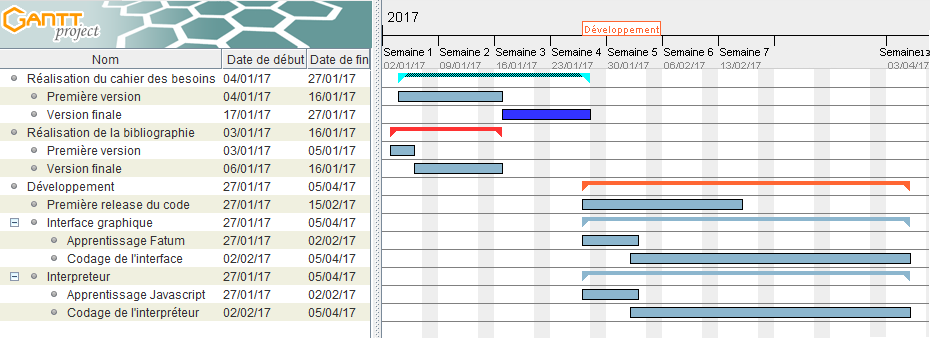
\includegraphics[width=1\textwidth]{images/GanttDiagram_edited.png}
    \caption{Diagramme de Gantt}
\end{figure}
\newpage
\bibliography{bibliographie}
\end{document}
